\documentclass[9pt]{article}
\usepackage{graphicx}
\usepackage{amsmath}
\usepackage[utf8]{inputenc}
\usepackage{titlesec}
\setcounter{secnumdepth}{4}
\usepackage{sectsty}
\usepackage[utf8]{inputenc}
\usepackage[T1]{fontenc}
\usepackage[a4paper, total={6in, 8in}]{geometry}
\renewcommand*\contentsname{Table of Contents}

\begin{document}

\begin{titlepage}
    \begin{center}
        \vspace*{1cm}
        
        \Huge
        \textbf{Control systems}
        
        \vspace{0.5cm}
        \LARGE
        Lab Project
        \vspace{0.5cm}
        
Modeling and Control of an indoor quadcopter\\
By\\
Mohan S P\\
Kenneth Joel 
        \vspace{0.8cm}
        
        
\includegraphics[width=0.4\textwidth]{university.jpg}
        
        \Large
        Department of Electrical and Electronics Engineering\\
        PES University\\
        Bengaluru-560085\\
    \end{center}
\end{titlepage}
 
\tableofcontents

\newpage

\part{Literature review}

\section{Objective}

To stabilize and control attitude (roll, pitch, yaw) and altitude of a quadcopter.

\section{Introduction}

A quadrotor helicopter (quadcopter) is a helicopter which has four equally spaced rotors. With four independent rotors, the need for a swash-plate mechanism is alleviated. The swash-plate mechanism was needed to allow the helicopter to utilize more degrees of freedom, but the same level of control can be obtained by adding two more rotors. The development of quadcopters has stalled until very recently, because controlling four independent rotors has proven to be incredibly difficult and impossible without electronic assistance. The decreasing cost of modern microprocessors has made electronic and even completely autonomous control of quadcopters feasible for commercial, military, and even hobbyist purposes. Quadcopter control is a fundamentally difficult and interesting problem. With $6$ degrees of freedom ($3$ translational and $3$ rotational) and only $4$ independent inputs (rotor speeds), quadcopters are severely under-actuated. In order to achieve $6$ degrees of freedom, rotational and translational motion are coupled. The resulting dynamics are highly nonlinear, especially after accounting for the complicated aerodynamic effects. Through this project we intend to implement a simplified controller for the quadcopter that should be capable of orientation stabilization and then orientation control which extends to linear motion as a result of the same.  

\section{Methodology}

\begin{itemize}
\item Literature survey
\item Obtain mathematical model of the drone considering process variables as roll, pitch and yaw.
\item Characterize the core-less DC Motors and design low form factor power circuit accordingly.
\item Design control circuit with specified micro-controller and implement the PID algorithm for the same.
\end{itemize}

\section{Assumptions in our model}

\subsection{Plus and cross configuration of the quadcopter}

\begin{center}
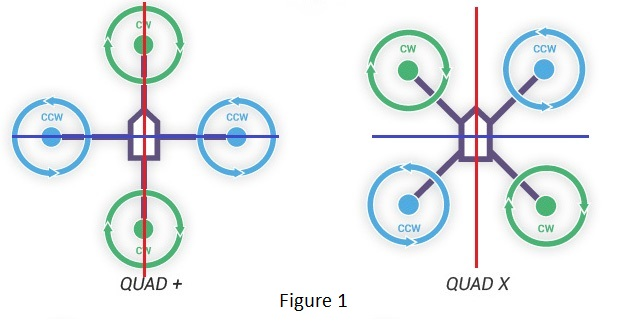
\includegraphics[width=1\textwidth]{1.jpg}
\end{center}

\noindent The first step to model a quadcopter would be to decide on a configuration. There are $2$ known configurations of quadcopter as shown in Figure $1$. Each with their advantages and disadvantages as follows:

\begin{itemize}

\item Rotational Moment: The rotational forces about roll and pitch axes of rotation for a $+$ system would be dependent on the thrust from only $1$ motor. In the case of the $X$ system the rotational forces would be dependent on any two motors, but the perpendicular distance from the axis of rotation is decreased by a factor of $\cos(\pi/4)$ in the case of a perfectly square arrangement of motors.

\item Camera arc clearance and visibility of yaw: These factors do not affect the modeling of the quadrotor but are significant considerations as they affect the user's convenience.

\end{itemize} 

\noindent However, there is no common consensus on whether either one of the two models are superior in an absolute sense from a practical standpoint. In terms of modelling the quadcopter there are not too many significant changes to be made as all changes can be accounted for in the thrust equations. The detailed differences between plus and cross configurations can be found in\cite{62431}

\subsection{Body axes system}

\begin{center}
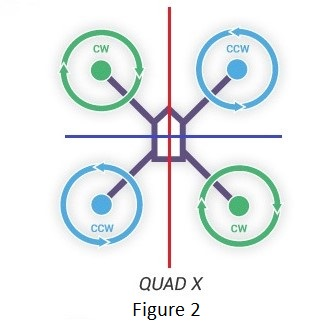
\includegraphics[width=0.4\textwidth]{2.jpg}
\end{center}

\noindent The body axis system we consider for this project is shown in Figure $2$ and is based on the cross configuration of the quadcopter. Also, the body axis center is assumed to be at the same position as the center of gravity.\\
Anticlockwise rotations are taken to be positive, the specifications for each axis and the displacements they correspond to are as follows:\\
Positive Pitch:	anticlockwise around $X$ axis $\rightarrow$ positive displacement in $Y$ direction\\
Positive Roll: anticlockwise around $Y$ axis $\rightarrow$ negative displacement in $X$ direction\\
Positive Yaw: anticlockwise around $Z$ axis $\rightarrow$ no net displacement\\
Increase in overall thrust $\rightarrow$ Positive displacement in $Z$ direction

\part{Mathematical Model}

\section{Motor Equations}

\begin{equation}
\tau = k_{t}(I-I_{o})
\end{equation}

\noindent $\tau$ : Torque\\
$k_{t}$	 : Torque proportionality constant\\ 
\noindent I	 : Current through the motor\\ 
$I_{o}$	 : No load current\\
		
\begin{equation}
V = IR_{m} + k_{v}\omega
\end{equation}						
		
\noindent V	 : Voltage Drop\\
$R_{m}$	 : Motor resistance\\
$k_{v}$	 : Back-emf/rpm proportionality constant\\

\begin{equation}
P = \frac{(\tau R_{m}+k_{t}I_{o}R_{m}+k_{v}k_{t}\omega)(\tau + k_{t}I_{o})}{k_{t}^2}
\end{equation}						
\noindent Approximating this equation by neglecting $R_{m}$ and considering $k_{t}I_{o} << \tau$ we get
 
\begin{equation}
P = \frac{k_{v}\tau\omega}{k_{t}}
\end{equation}						

\noindent By conservation of energy, we know that the energy the motor expends in a given time period is equal to the force generated on the propeller times the distance that the air it displaces moves. Therefore

\begin{eqnarray}
P \cdot dt=T \cdot dx\\
P=Tv_{h}\\
\frac{k_{v}\tau\omega}{k_{t}}=Tv_{h}
\end{eqnarray}

\noindent $v_{h}$ : Hover Velocity\\

\noindent From Aerodynamics we have

\begin{equation}
v_{h} = \sqrt{\frac{T}{2 \rho A}}
\end{equation}				

\noindent Using this we can rewrite the power equation as
\begin{equation}
P = \frac{T^{3/2}}{\sqrt{2 \rho A}}
\end{equation}
						
\noindent T : Thrust\\
$\rho$ : Air Density \\
A : Area swept by the propeller\\

\noindent We know that torque is proportional to thrust. Therefore
\begin{equation}
\tau = k_{\tau}T
\end{equation}

\noindent $k_{\tau}$ : Thrust proportionality constant\\

\noindent Note: For our project we consider uniform density of air $\rho$ since the drone flies within a limited space.\\ 

\noindent Substituting ($10$) in ($4$) and equating it to ($9$) we get

\begin{equation}
T = \left(\frac{\omega k_{v} k_{\tau} \sqrt{2 \rho A}}{k_{t}}\right)^{2}
\end{equation}

\noindent The only variable is $\omega$. Therefore ($11$) becomes

\begin{equation}
T = k\omega^{2}
\end{equation}

\noindent Since there are $4$ motors equation ($12$) becomes 

\begin{eqnarray}
T_{B} = 
\left[
\begin{matrix}
0 \\
0 \\
k(\omega_{1}^{2} + \omega_{2}^{2} + \omega_{3}^{2} + \omega_{4}^{2})  
\end{matrix}
\right]
\end{eqnarray}

\section{Drag Forces}

\noindent The matrix below describes drag forces in $3$ directions

\begin{eqnarray}
F_{d} =
\left[
\begin{matrix}
-k_{d}\dot{x} \\
-k_{d}\dot{y} \\
-k_{d}\dot{z}
\end{matrix}
\right]
\end{eqnarray}

\noindent $k_{d}$ : Drag co-efficient \\
$\dot{x}$ , $\dot{y}$ , $\dot{z}$ : Linear velocities in x , y , z directions respectively. \\

\noindent From fluid dynamics we have
 
\begin{equation}
F_{D} = \frac{\rho C_{D}Av^{2}}{2}
\end{equation}

\noindent Therefore $\tau_{D}$ can be written as

\begin{equation}
\tau_{D} = \frac{\rho R^{3} C_{D}A \omega^{2}}{2}
\end{equation}

\noindent The only variable is $\omega$. Therefore ($16$) becomes

\begin{equation}
\tau_{D} = b\omega^{2}
\end{equation}
 
\noindent $C_{D}$ : Drag Constant \\
v : Linear Velocity

\section{Torques}
\noindent According to our model the roll, pitch and yaw torques can be represented as

\begin{eqnarray}
\left[
\begin{matrix}
\tau_{\phi}\\
\tau_{\theta}\\
\tau_{\psi}
\end{matrix}
\right]=
\left[
\begin{matrix}
Lk\sqrt{2} (\omega_{2}^{2} + \omega_{3}^{2} - \omega_{1}^{2} - \omega_{4}^{2}) \\
Lk\sqrt{2} (\omega_{3}^{2} + \omega_{4}^{2} - \omega_{1}^{2} - \omega_{2}^{2}) \\
b(\omega_{1}^{2} - \omega_{2}^{2} + \omega_{3}^{2} - \omega_{4}^{2})
\end{matrix}
\right]=
\tau_{B}
\end{eqnarray}

\noindent L : Boom length\\

\noindent Expressing linear motion in the inertial frame we get

\begin{eqnarray}
\ddot{a} =
\left[
\begin{matrix}
0 \\
0 \\
-g
\end{matrix}
\right]+
\left[
\begin{matrix}
\frac{RT_{B}}{m}
\end{matrix}
\right]+
\left[
\begin{matrix}
\frac{F_{d}}{m}
\end{matrix}
\right]
\end{eqnarray}

\begin{eqnarray}
\ddot{a} = 
\left[
\begin{matrix}
\ddot{x} \\
\ddot{y} \\
\ddot{z} 
\end{matrix}
\right]
\end{eqnarray}

\begin{eqnarray}
R =
\left[
\begin{matrix}
c_{\theta}c_{\psi} & c_{\theta}s_{\psi} & -s_{\theta}   \\
s_{\phi}s_{\theta}c_{\psi}-c_{\phi}s_{\psi} & c_{\phi}c_{\psi}+s_{\phi}s_{\theta}s_{\psi} & c_{\theta}s_{\phi}   \\
s_{\phi}s_{\psi}+c_{\phi}s_{\theta}c_{\psi} & c_{\phi}s_{\theta}c_{\psi}-s_{\phi}c_{\psi} & c_{\phi}c_{\theta}
\end{matrix}
\right]
\end{eqnarray}

\section{Euler's Equation for Rotational Motion}

Euler expressed rotational motion in the body frame using the following equation\cite{68291}

\begin{equation}
\tau_{B} = I\dot{\omega} + (\omega \times I\omega) 
\end{equation}

\noindent I : Moment of Inertia

\begin{eqnarray}
I =
\left[
\begin{matrix}
I_{xx} & 0 & 0 \\
0 & I_{yy} & 0 \\
0 & 0 & I_{zz}
\end{matrix}
\right]
\end{eqnarray}

\begin{eqnarray}
\omega = 
\left[
\begin{matrix}
\omega_{x} \\
\omega_{y} \\
\omega_{z} \\
\end{matrix}
\right]
\end{eqnarray}

\noindent From ($22$) we get

\begin{equation}
\dot{\omega}=I^{-1}(\tau - (\omega \times (I\omega)))
\end{equation}

\noindent Therefore by substituting ($18$) ($23$) and ($24$) in ($25$) we get 

\begin{eqnarray}
\dot{\omega} =
\left[
\begin{matrix}
\tau_{\phi}I_{xx}^{-1} - \frac{(I_{yy}-I_{zz})\omega_{y}\omega_{z}}{I_{xx}} \\
\tau_{\theta}I_{yy}^{-1} - \frac{(I_{zz}-I_{xx})\omega_{z}\omega_{x}}{I_{yy}} \\
\tau_{\psi}I_{xx}^{-1} - \frac{(I_{yy}-I_{zz})\omega_{x}\omega_{y}}{I_{zz}} 
\end{matrix}
\right]
\end{eqnarray}

\section{State Space Model}

To describe a quadcopter in space we need the following variables in all $3$ axes:
\begin{itemize}
\item Position
\item Linear velocities
\item Orientation
\item Angular velocities
\end{itemize}

\noindent This comes upto $12$ variables and can be represented as follows

\begin{eqnarray}
\left[
\begin{matrix}
x \\
y \\
z \\
\dot{x} \\
\dot{y} \\
\dot{z} \\
\phi \\
\theta \\ 
\psi \\
\omega_{x} \\
\omega_{y} \\
\omega_{z}  
\end{matrix}
\right]
\end{eqnarray}

\noindent We can assume $4$ vectors $x_{1}$ $x_{2}$ $x_{3}$ $x_{4}$ such that

\begin{eqnarray}
x_{1} =
\left[
\begin{matrix}
x \\
y \\
z \\
\end{matrix}
\right]
\end{eqnarray}

\begin{eqnarray}
x_{2} =
\left[
\begin{matrix}
\dot{x} \\
\dot{y} \\
\dot{z}
\end{matrix}
\right]
\end{eqnarray}

\begin{eqnarray}
x_{3} =
\left[
\begin{matrix}
\phi \\
\theta \\ 
\psi
\end{matrix}
\right]
\end{eqnarray}

\begin{eqnarray}
x_{4} =
\left[
\begin{matrix}
\omega_{x} \\
\omega_{y} \\
\omega_{z}
\end{matrix}
\right]
\end{eqnarray}

\begin{equation}
\dot{x_{4}} = x_{2}
\end{equation}

\begin{eqnarray}
\dot{x_{2}} =
\left[
\begin{matrix}
0 \\
0 \\
-g
\end{matrix}
\right]+
\frac{RT_{B}}{m} + F_{d}
\end{eqnarray}

\begin{eqnarray}
\dot{x_{3}} = 
\left[
\begin{matrix}
1 & -t_{\theta}s_{\phi} & -c_{\phi}t_{\theta}   \\
0 & c_{\phi} & -s_{\phi}   \\
0 & \frac{s_{\phi}}{c_{\theta}} & \frac{c_{\phi}}{s_{\theta}}
\end{matrix}
\right]
x_{4}
\end{eqnarray}

\begin{eqnarray}
\dot{x_{4}} =
\left[
\begin{matrix}
\tau_{\phi}I_{xx}^{-1} - \frac{(I_{yy}-I_{zz})\omega_{y}\omega_{z}}{I_{xx}} \\
\tau_{\theta}I_{yy}^{-1} - \frac{(I_{zz}-I_{xx})\omega_{z}\omega_{x}}{I_{yy}} \\
\tau_{\psi}I_{xx}^{-1} - \frac{(I_{yy}-I_{zz})\omega_{x}\omega_{y}}{I_{zz}} 
\end{matrix}
\right]
\end{eqnarray}

\part{Simulation}
While surveying potential options for simulation of the quadrotor system as a whole the following were considered:

\begin{itemize}
\item Using asbQuadCopter Simulink library.
\item Importing a 3D CAD model of the quadcopter from solidworks into Simulink as an XML File using sim-import.
\item Developing a basic simulation from ground up.
\item Adopting some open source models to suit our needs.
\end{itemize}

\noindent We chose to adopt an open source model designed by MEM students of Drexell university to suit our requirements for this project. Doing this we gained significant exposure to tools that we were unfamiliar with as well as a good sense of structure and modularity.\\
However, the other techniques listed are also quite useful and are adopted for several commercial products and should be considered as future improvements.\\
The figure below shows the model we used as displayed in simulink containing the four main masked subsystems and four action buttons. Their roles are as labeled in the image.\\

\begin{center}
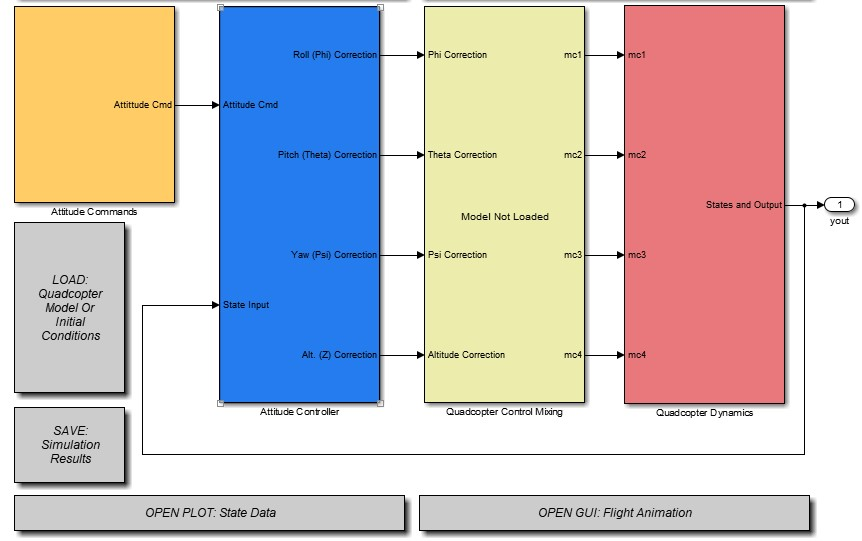
\includegraphics[width=0.87\textwidth]{8.jpg}
\end{center}

\section{Attitude command}
\noindent Expanding the first subsystem (yellow) reveals the model as shown in the figure above which represents the inputs specified by the user given by corresponding step inputs for roll pitch yaw and altitude.

\begin{center}
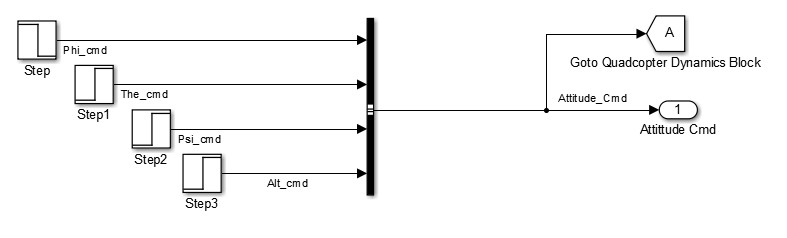
\includegraphics[width=0.87\textwidth]{9.jpg}
\end{center}

\noindent Expanding the second subsystem (blue) reveals the model shown in the figure above which comprises of four PID controllers working in parallel to issue correction commands for each corresponding action to the next block. The controllers are implemented as masked function blocks with parameters that can be defined as shown in the figure below.

\begin{center}
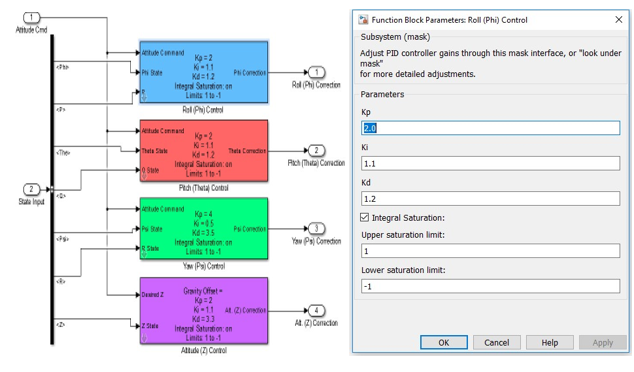
\includegraphics[width=0.86\textwidth]{10.jpg}
\end{center}

\section{Control mixing}

\begin{center}
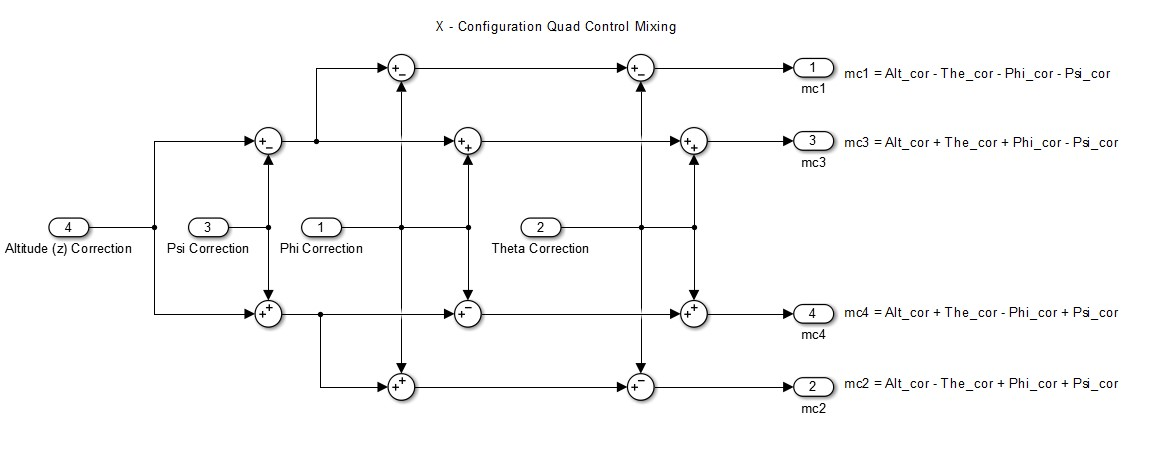
\includegraphics[width=0.8\textwidth]{11.jpg}
\end{center}

\noindent Expanding the third subsystem (blue) reveals the model shown in the figure above which as labeled is the motor control mixing based on correction commands given by the controller for a cross configured quadrotor.

\section{Quadcopter dynamics}

\begin{center}
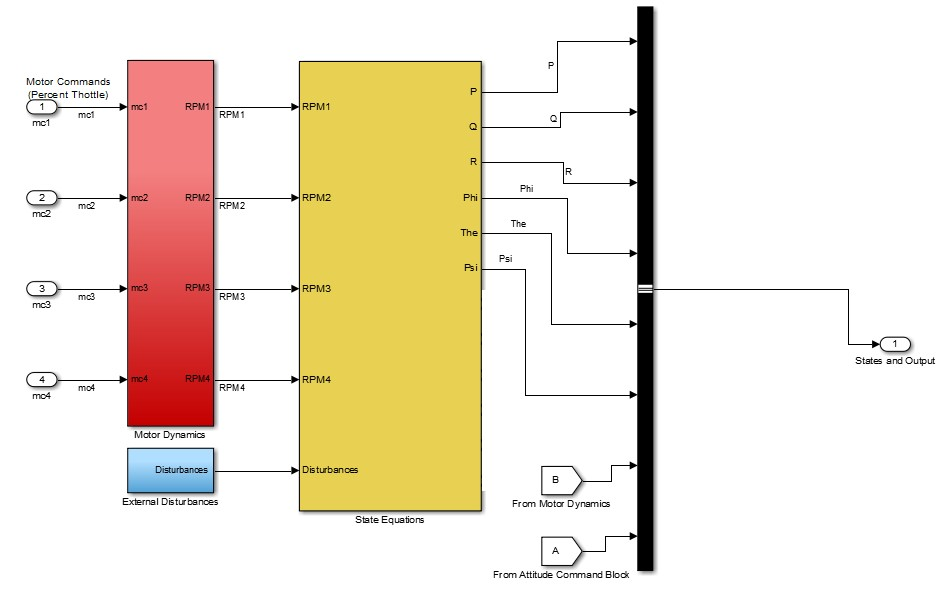
\includegraphics[width=0.8\textwidth]{12.jpg}
\end{center}

\noindent Expanding the third subsystem (blue) reveals the model shown in the figure above. The red block represents the motor dynamics and the yellow block is defined by a level $2$ S-function which implements the mathematical model of the system. We have used the mathematical model we derived in Part II Section 9 in this S function. However, we have not considered states involving position and velocity since for this project we are primarily concerned with the orientation of the quadcopter. Majority of the modifications made were in this section of the model. 

\subsection{S-function code}

\begin{flushleft}

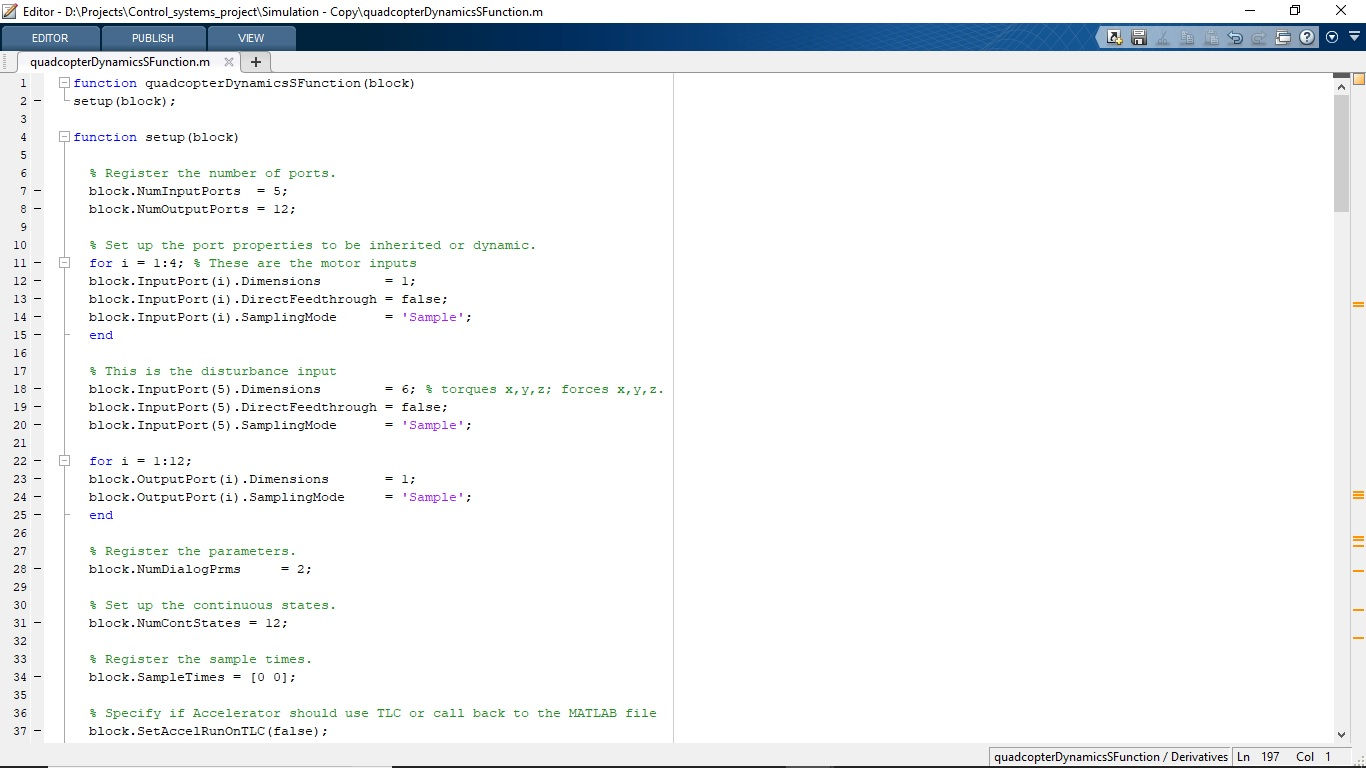
\includegraphics[width=175mm,height=165mm]{18.jpg}
\newpage
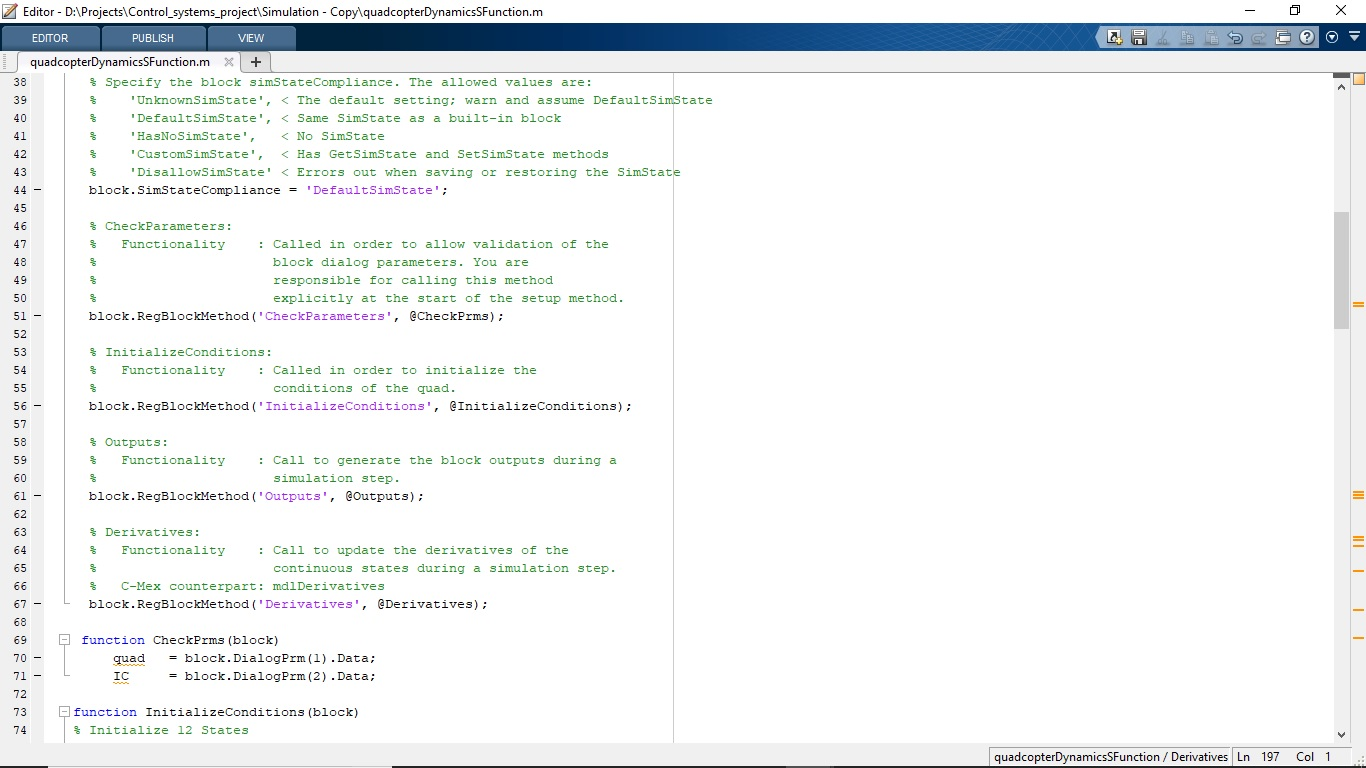
\includegraphics[width=175mm,height=165mm]{19.jpg}
\newpage
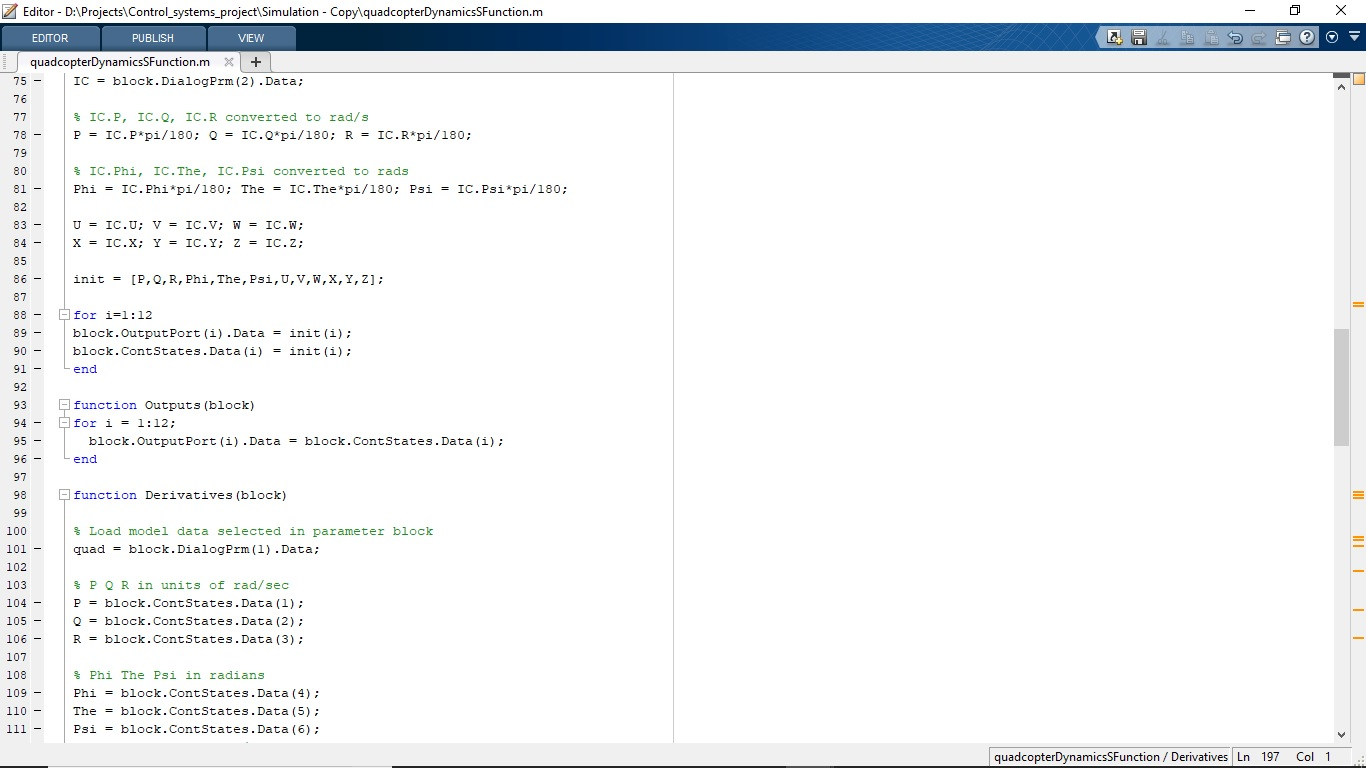
\includegraphics[width=175mm,height=165mm]{20.jpg}
\newpage
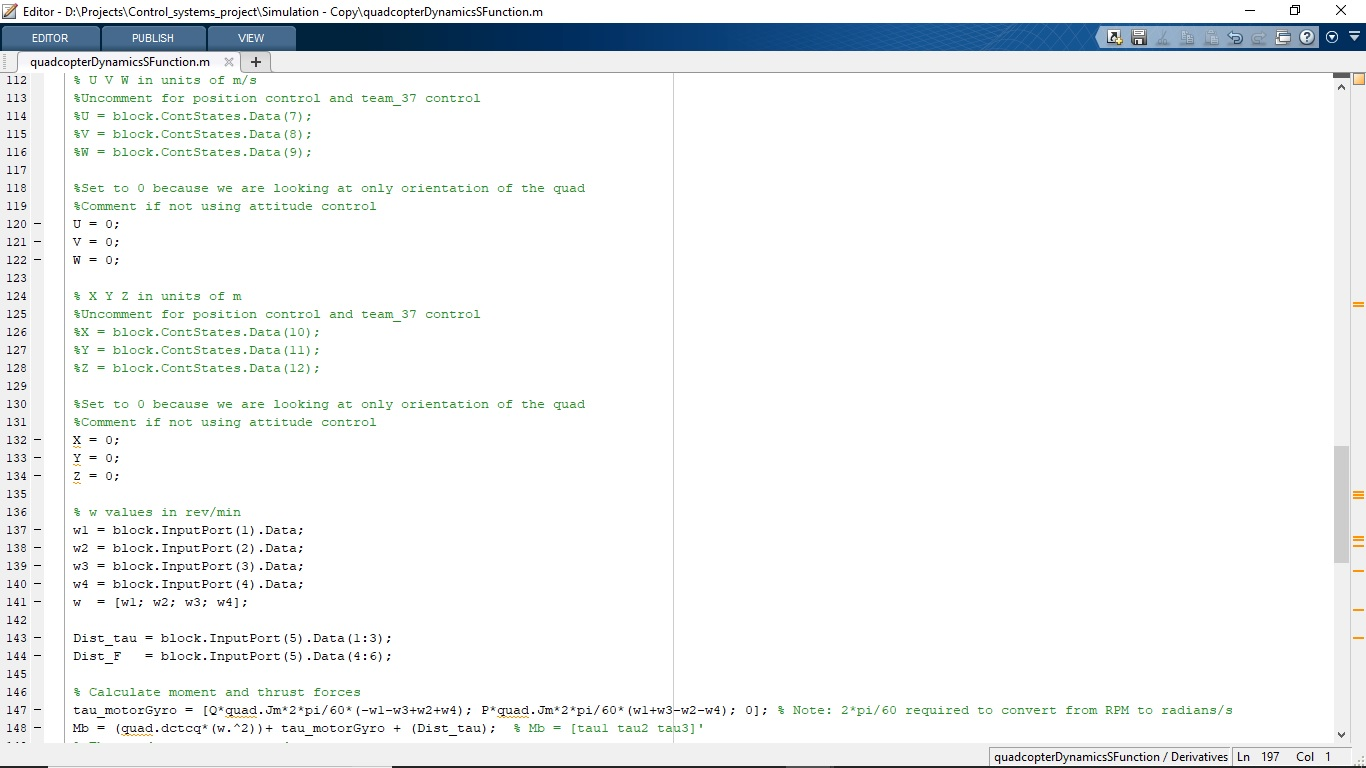
\includegraphics[width=175mm,height=165mm]{21.jpg}
\newpage
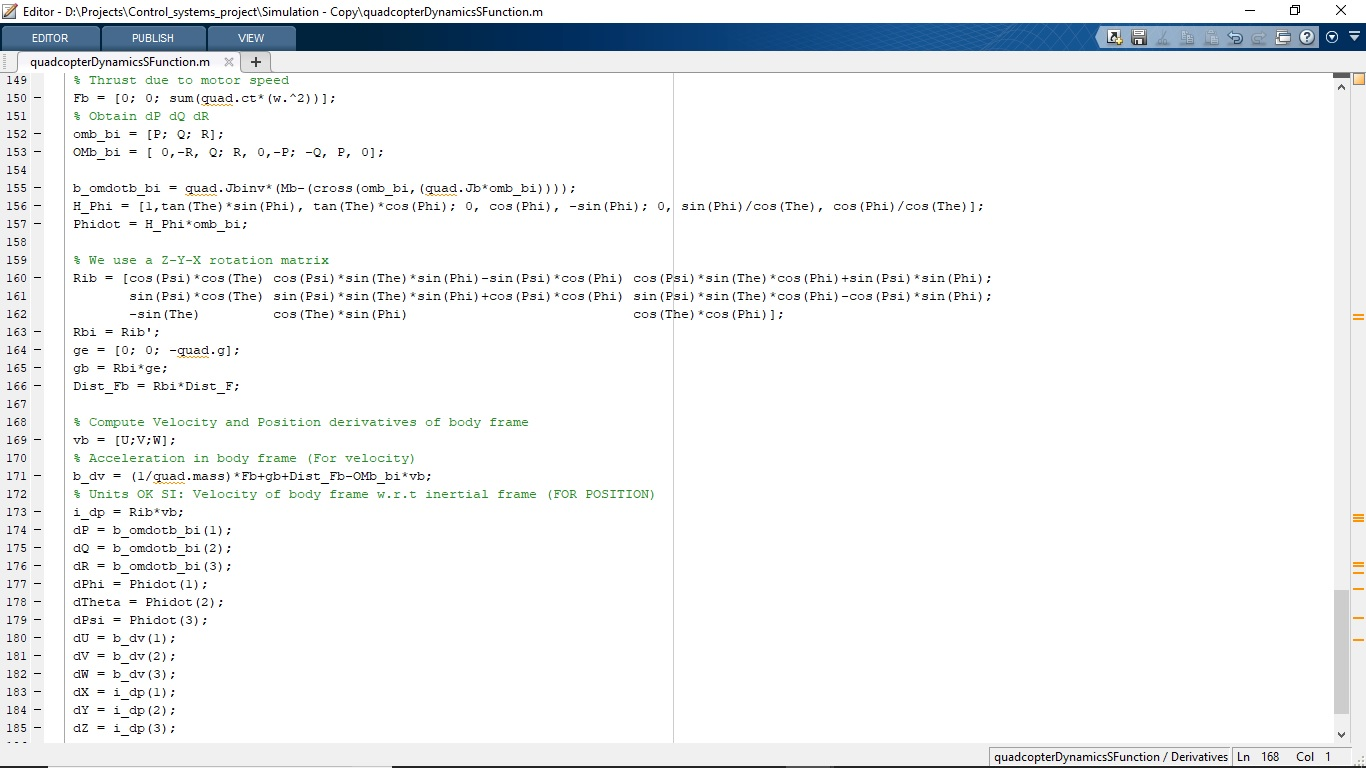
\includegraphics[width=175mm,height=165mm]{22.jpg}

\end{flushleft}

\section{Loadable files}

\begin{center}
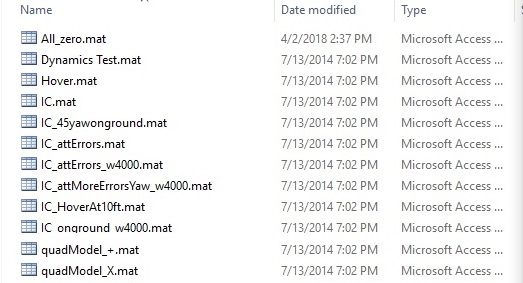
\includegraphics[width=0.8\textwidth]{13.jpg}
\end{center}

\noindent As seen in the left half of the above figure the simulation allows us to load predefined configuration files or initial condition files to the model. These files are used either to define a quadcopter model or initialize the state variables to some initial conditions before the execution of the simulation. For our purposes we use only \texttt{quadModel\_X.mat} since we have modeled a cross configured quadcopter. Initial conditions were defined as per our needs in the simulation, note that even here we define initial conditions that affect the orientation of the quadcopter and nothing that affects translation or absolute position as that is out of the scope of this project.

\section{Sample output}
\noindent Action Buttons ‘OPEN PLOT: State Data’ and ‘OPEN GUI: Flight Animation’ give us the plots and $3$D animation respectively.

\subsection{OPEN PLOT: State Data}

\begin{center}
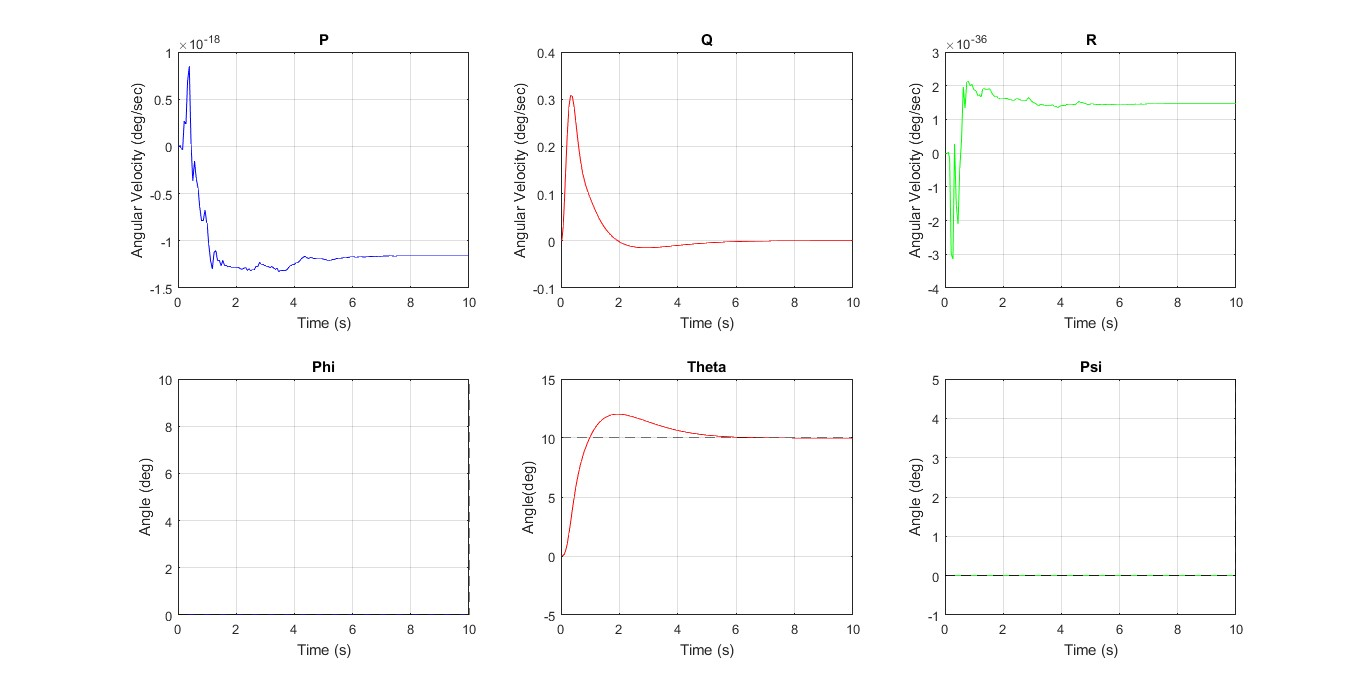
\includegraphics[width=0.8\textwidth]{14.jpg}
\end{center}

\begin{center}
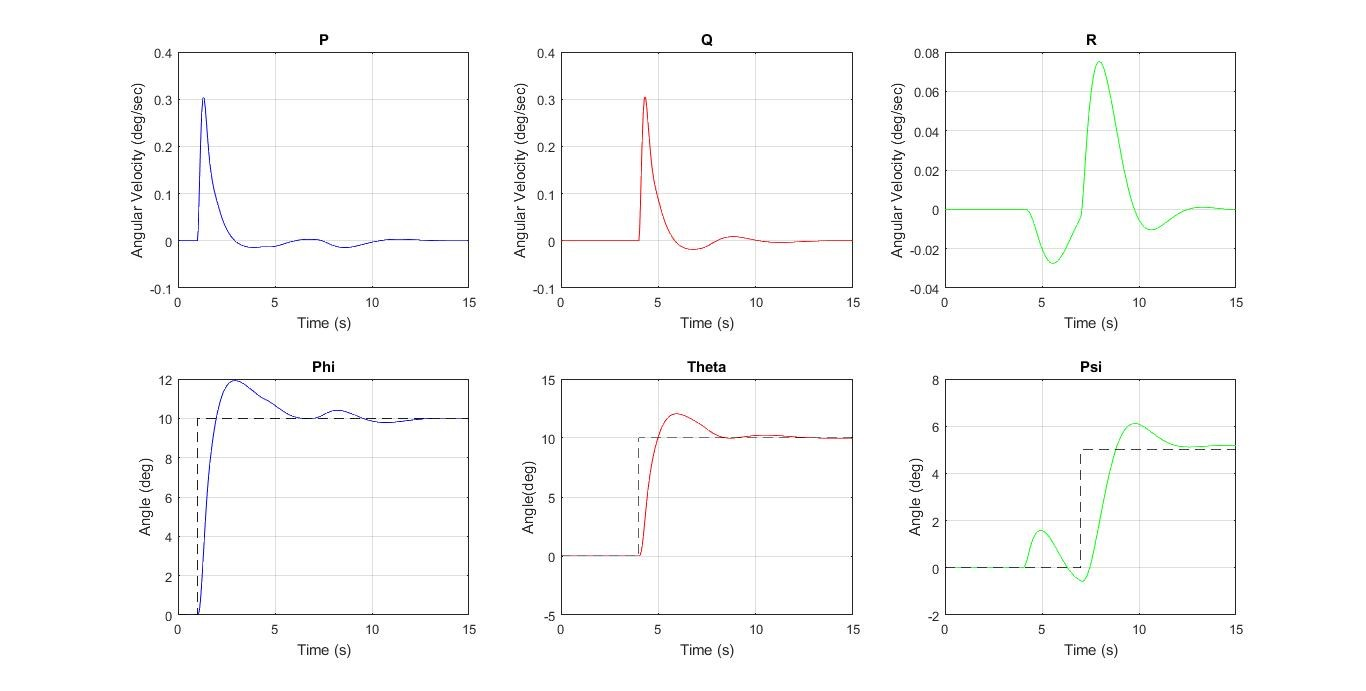
\includegraphics[width=1.0\textwidth]{16.jpg}
\end{center}

\noindent The plots shown above correspond to angle [$\phi$, $\theta$, $\psi$] and angular velocity [$P$, $Q$, $R$] of the quadcopter about all the axes. This is a result of the output obtained for the previous block which gave the state data. We are primarily concerned with the plots of angle vs time and hope for a slightly underdamped response in these cases.\\ \\
The first plot shows the response response of the system to a 10$^\circ$ step input to $\theta$ at $t=0$\\
The second plot shows the response of the system to hybrid inputs at different points in time.

\subsection{OPEN GUI: Flight Animation}

\begin{center}
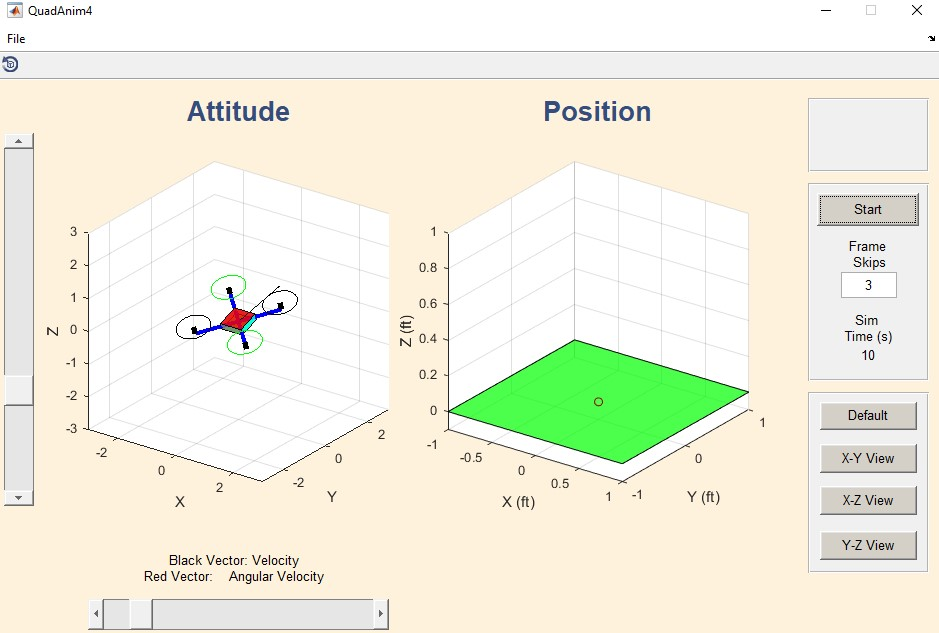
\includegraphics[width=0.45\textwidth]{15.jpg}
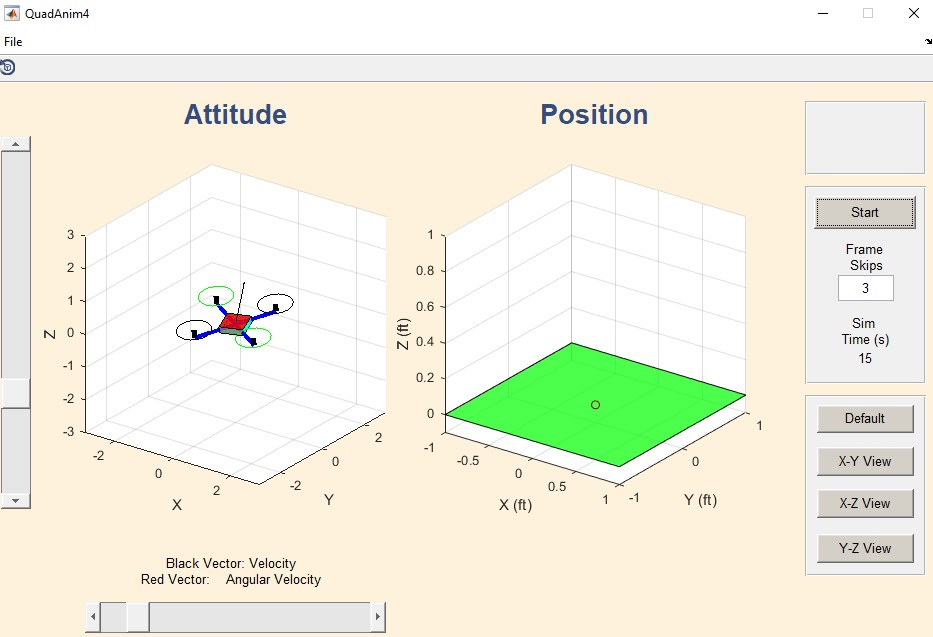
\includegraphics[width=0.45\textwidth]{17.jpg}
\end{center}

\noindent The 3D animation gives us visual information about the orientation and position of the quadcopter in 3D space, for this project we have not allowed the quadcopter to translate in space so we are primarily concerned with the orientation (shown on the left side of the above figures). \\ \\
The first figure shows the response of the system to a 10$^\circ$ step input to $\theta$ at $t=0$\\
The second figure shows the response of the system to hybrid inputs at different points in time.

\part{Hardware}

\section{Motor characterization}

\noindent The motor we will be using for this project is the one shown in Figure $3$. These type of motors are called core-less motor. The main reason behind using these motors is because they can generate very high rpm at very low voltages.

\begin{center}
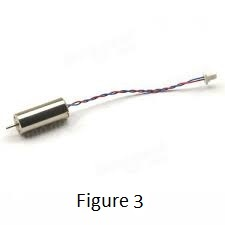
\includegraphics[width=0.4\textwidth]{3.jpg}
\end{center}

\noindent The characterization of this motor was done to figure out the relation between Voltage and Current and Voltage and Thrust. The results obtained are as shown below.

\begin{center}
\begin{tabular}{ |p{1.3cm}|p{1.3cm}|p{1.9cm}|}
\hline
$Volts (V)$ & $Amps (A)$ & $Thrust (g cm)$\\
\hline
3.3 & 0.96 & 18.36 \\
3.4 & 1.00 & 18.71 \\
3.5 & 1.04 & 20.01 \\
3.6 & 1.09 & 21.04 \\
3.7 & 1.13 & 21.73 \\
3.8 & 1.18 & 23.06 \\
3.9 & 1.22 & 23.28 \\     
\hline
\end{tabular}
\end{center}

\begin{center}
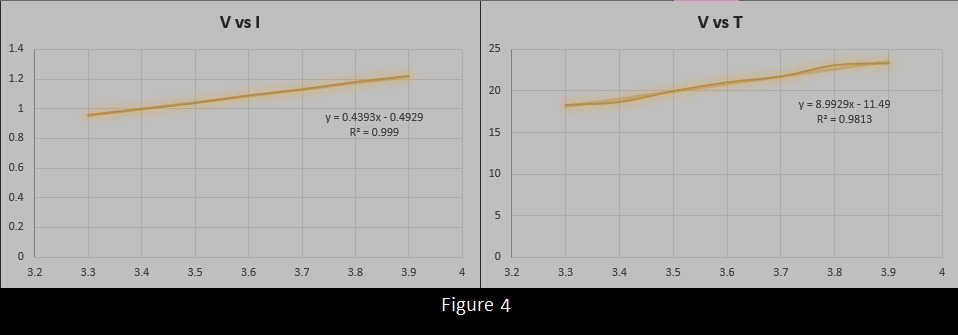
\includegraphics[width=0.9\textwidth]{4.jpg}
\end{center}

From Figure $4$ we can conclude the relation between the analyzed quantities as follows.

\begin{equation}
I = (0.4393 * V) - 0.4929
\end{equation}

\begin{equation}
T = (8.9929 * V) - 11.49
\end{equation}
 
These equations were obtained using Microsoft Excels built-in curve fitting feature.  

\section{Inertial Measurement Unit (MPU6050)}

\begin{center}
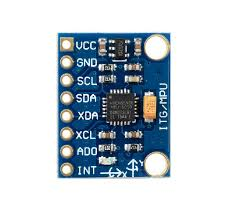
\includegraphics[width=0.4\textwidth]{5.jpg}
\end{center}

\noindent This sensor is intended to be used to measure the absolute orientation of an object. MPU6050 is an integration of these $2$ sensors:
\begin{itemize}
\item Accelerometer
\item Gyroscope
\end{itemize}
 
\noindent It has an on board Digital Motion Processor to evaluate motion fusion operations. To summarize their individual operations:

\begin{itemize}

\item Accelerometer\\
Used to measure the components of linear acceleration of the object in $3$ dimensions with respect to the body axes of the sensor.

\item Gyroscope\\
Used to measure the angular rate of change of the object with respect to the body axes of the sensor.

\end{itemize}

\noindent The unique combination of these $2$ sensors is what enables us to obtain the absolute orientation of the drone in $3$D space, this introduces feedback to the plant by giving us real time information about the orientation of the drone. Our PID algorithm will evaluate errors based on outputs from this sensor.\\

\section{Driver circuit}
The driver circuit that works best for the coreless motors we are using, is the one shown in the figure above. The circuit allows unidirectional control of the motor using the PWM signal from the Arduino that is then amplified by the MOSFET.\\

\begin{center}
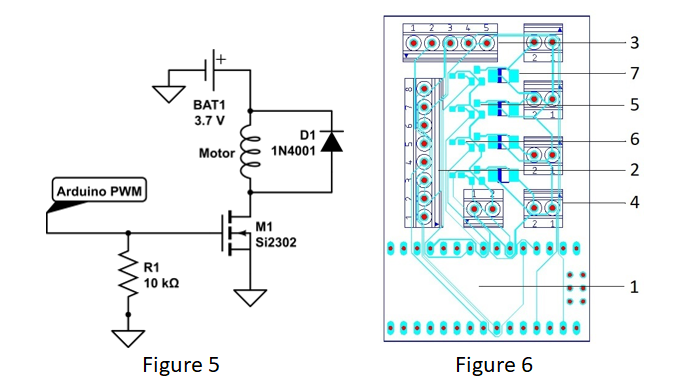
\includegraphics[width=0.8\textwidth]{6.jpg}
\end{center}

\begin{center}
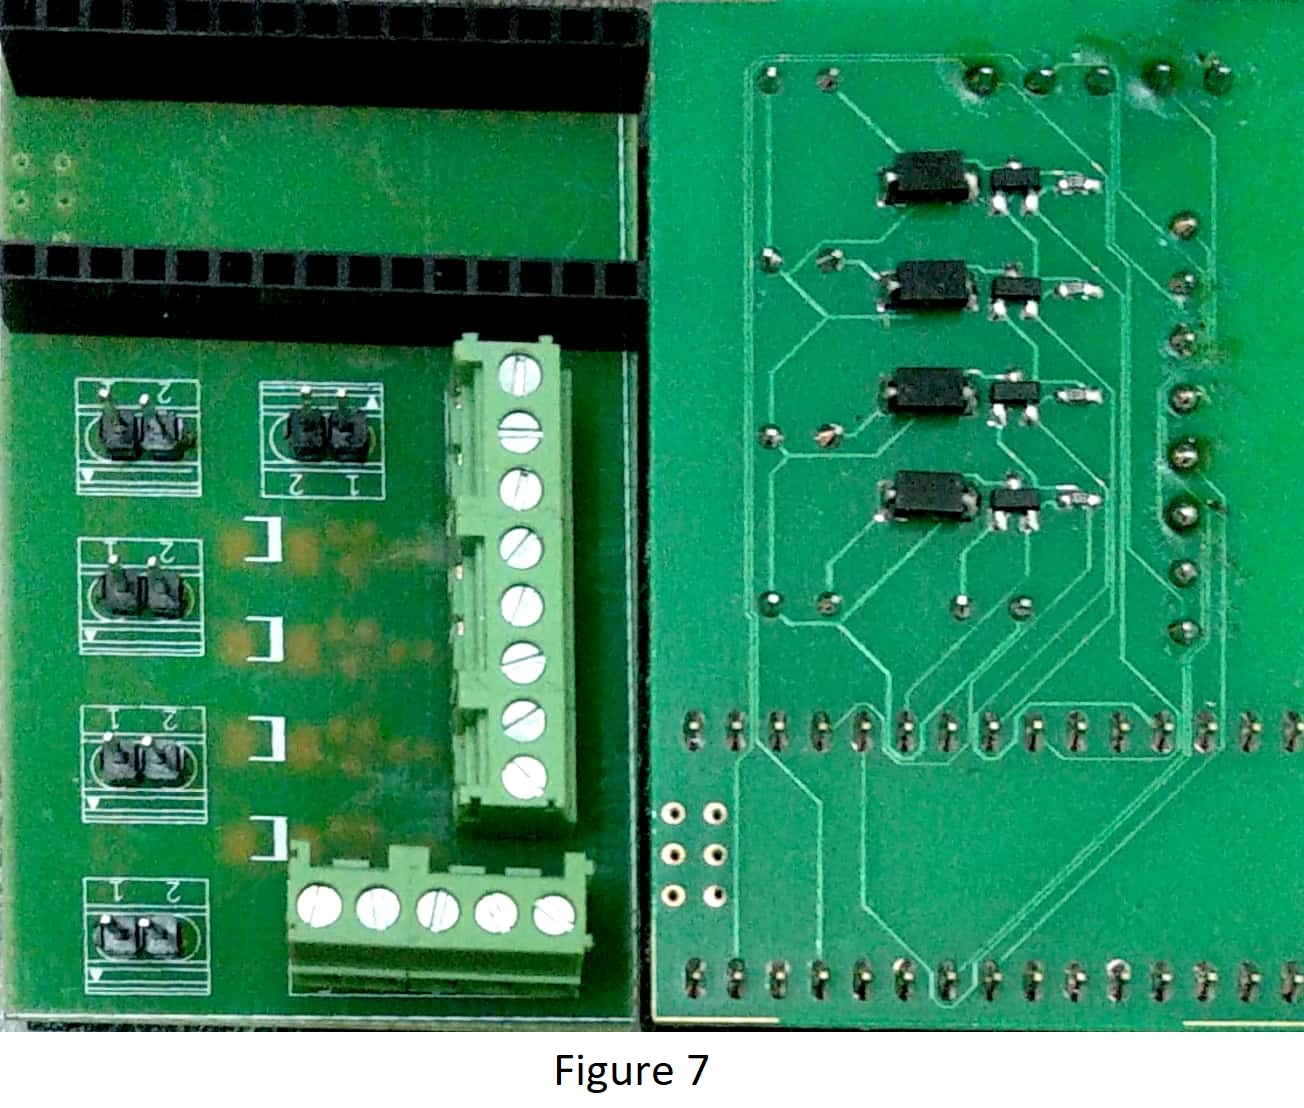
\includegraphics[width=0.7\textwidth]{7.jpg}
\end{center}

\noindent Figure $5$ shows the schematic for a single brushless motor. For our application we need 4 identical circuits to control the four motors independently. To facilitate this a PCB was fabricated that\\ accommodates the controller, sensors and driver circuit on the same board (as shown in Figure $6$).\\ \\
Figure $7$ shows the fabricated board. The components used in the fabricated board are as follows:

\begin{enumerate}
\item Main Controller (Arduino Nano)
\item Accelerometer + Gyroscope (MPU6050)
\item Compass (HMC5883)
\item Motor Output Pins
\item SMD Logic Level MOSFET (Si2302, SOT-23/TO-236)
\item 10k resistors (0603)
\item Freewheeling Diode (IN4001, DO-214AC) \\
\end{enumerate}
 
\subsection{Justification for the components}
\begin{itemize}
\item Arduino Nano\\
We chose this microcontroller to carry out the task of stabilization of drone. We have implemented a PID control for attitude stabilization of the drone. This was the best microcontroller which satisfied our memory, power and form factor requirements.

\item MPU6050\\
We first experimented with MPU9250 which had Accelerometer$+$Gyroscope$+$Magnetometer. We realized that the yaw given by the sensor was not reliable. Therefore we decided to go for MPU6050 and use relative yaw instead of absolute yaw.

\item Si2302\\
The reason why we went for this logic level MOSFET is because it can be easily gated by the output pins of Arduino Nano without the help of any external gating circuit. The current rating of this MOSFET was also appropriate for our application. The reason for choosing the SMD version is to reduce the form-factor of the PCB.

\item $10$k resistor\\
This resistor is used to limit the gate current flowing into the MOSFET incase of an overshoot. SMD version has been chosen to reduce the form-factor of the PCB.

\item $1$N$4001$\\
This diode is used a free-wheeling diode to protect the circuit from inductive fly-back effect of the motor. SMD version has been chosen to reduce the form-factor of the PCB.
   
\end{itemize}
\noindent Efforts were made to reduce the form factor by as much as possible. To make the circuit board more robust, tracks that carry high current were made twice as thick as tracks use for logic connections.
 
\section{Test rig}
The quadcopter is connected to mount which is connected to a spherical joint which is connected to a base gives it all required degrees of freedom (as shown in Figure $8$). However our quad was too heavy to use this mount. Therefore in order to test the quad we used the same mount but suspended using a thread (as shown in Figure $9$) giving us the ability to test yaw. We were able to test roll and pitch also to a certain extent.

\begin{center}
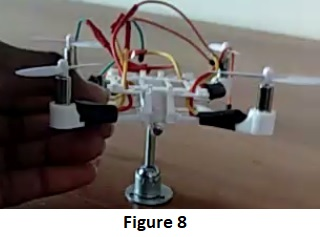
\includegraphics[width=0.6\textwidth]{31.jpg}
\end{center}

\begin{center}
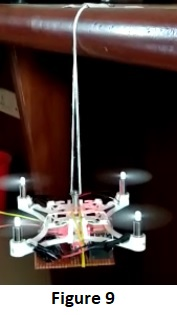
\includegraphics[width=0.37\textwidth]{32.jpg}
\end{center}

\part{Control}

\section{Control considerations}

A typical global coordinate system based trajectory planning set up would have goals specified according to a start and end point, or some curve expressing the trajectory to be followed. To successfully implement such a system we would need to design a controller with the following process variables:\\

\begin{itemize}
\item Position
\item Linear velocity
\item Angular velocity
\item Linear acceleration
\item Angular acceleration
\item Jerk
\item Snap
\end{itemize}

\noindent This results in a very complex model that is hard to compute in real time. Also, some of these parameters cannot even be accurately measured with existing sensor technology. This makes the approach practically unfeasible though mathematically robust.\\ \\

\noindent It is very common to find roll, pitch, yaw and altitude control in a parallel PID setup, as this is the most feasible in terms of physical implementation, due to its inherent simplicity and the coupling that these rotational changes and translation motion have. The disadvantage of this is that the operator of the quadcopter would now need to be consciously manipulating these parameters in order to obtain his desired trajectory.\\ \\
However, in autonomous systems it is common to find another layer of control implemented to plan trajectories by manipulating roll pitch yaw and altitude. A sort of multilevel structure simplifies the problem mathematically while giving us the same results as the case described previously. From a control systems perspective we can look at this system as one that is controlled by a cascaded PID.\\ \\
Though most of this is out of the scope of what we intend to achieve we think it is important to understand this distinction and the limitations associated with it.

\newpage

\section{Mathematical Implementation}

Here we use a simple PID controller to control [$\phi$ $\theta$ $\psi$]. These values are read in real time from MPU6050.\\

\noindent Note: If required altitude control can also be implemented in this by using BMI180 pressure sensor to detect the z co-ordinate in an absolute sense.\\

\noindent We know that 
\begin{equation}
\tau = Iu(t)
\end{equation}

\noindent u(t) : Input to the system\\

\noindent Since we are implementing a PID control the input depends on the error. According to the equations of the PID controller we get

\begin{eqnarray}
\left[
\begin{matrix}
\tau_{\phi} \\
\tau_{\theta} \\
\tau{\psi} 
\end{matrix}
\right]=
\left[
\begin{matrix}
-I_{xx}(k_{p}e_{\phi} + k_{d}\dot{e_{\phi}} + k_{i}$$\int_{}^{} e_{\phi} dt$$\\
-I_{yy}(k_{p}e_{\theta} + k_{d}\dot{e_{\theta}} + k_{i}$$\int_{}^{} e_{\theta} dt$$\\
-I_{zz}(k_{p}e_{\psi} + k_{d}\dot{e_{\psi}} + k_{i}$$\int_{}^{} e_{\psi} dt$$
\end{matrix}
\right]
\end{eqnarray}

\noindent For simplicity assume
\begin{equation}
\gamma_{i}=\omega_{i}^{2}
\end{equation}
\\
\noindent From ($18$) and ($39$) we get\\

\begin{eqnarray}
\left[
\begin{matrix}
\gamma_{2} + \gamma_{3} - \gamma_{1} - \gamma_{4} \\
\gamma_{3} + \gamma_{4} - \gamma_{1} - \gamma_{2} \\
\gamma_{1} - \gamma_{2} + \gamma_{3} - \gamma_{4}\\ 
\end{matrix}
\right]=
\left[
\begin{matrix}
\frac{I_{xx}(k_{p}e_{\phi} + k_{d}\dot{e_{\phi}} + k_{i} \int_{}^{}e_{\phi}dt)}{Lk\sqrt{2}}  \\
\frac{I_{yy}(k_{p}e_{\theta} + k_{d}\dot{e_{\theta}} + k_{i} \int_{}^{}e_{\theta}dt)}{Lk\sqrt{2}} \\
\frac{I_{zz}(k_{p}e_{\psi} + k_{d}\dot{e_{\psi}} + k_{i} \int_{}^{}e_{\psi}dt)}{b} \\
\end{matrix}
\right]
\end{eqnarray}

\noindent From the above equations we have $4$ unknowns and $3$ equations. Therefore in order to calculate the $4$ unknowns we can add a constraint T=mg.\\

\noindent Projecting it onto the inertial frame we get

\begin{equation}
T=\frac{mg}{c_{\theta}c_{\phi}}
\end{equation}

\noindent This implies

\begin{equation}
\gamma_{1} + \gamma_{2} + \gamma_{3} + \gamma_{4}=\frac{mg}{c_{\theta}c_{\phi}}
\end{equation}

\noindent In order to obtain the input equations for the speed of the four motors equations ($41$) and ($43$) has to be solved.

\section{Practical implementation}
\noindent The PID controller is implemented on a micro-controller. This project requires $3$ parallel PIDs for roll pitch and yaw respectively followed by control mixing for a cross configuration quadcopter.
The error variable considered here is the R-P-Y angles in degrees obtained from the sensor (MPU6050). The initial calibration routine runs for 15 seconds during which the yaw drift settles and the current position of the quadcopter corresponds to 0 degrees in all degrees of freedom. In the implementation of the PID time taken for each iteration is measured and used to calculate differential and integral error terms.

\subsection{Arduino Code}

\begin{flushleft}

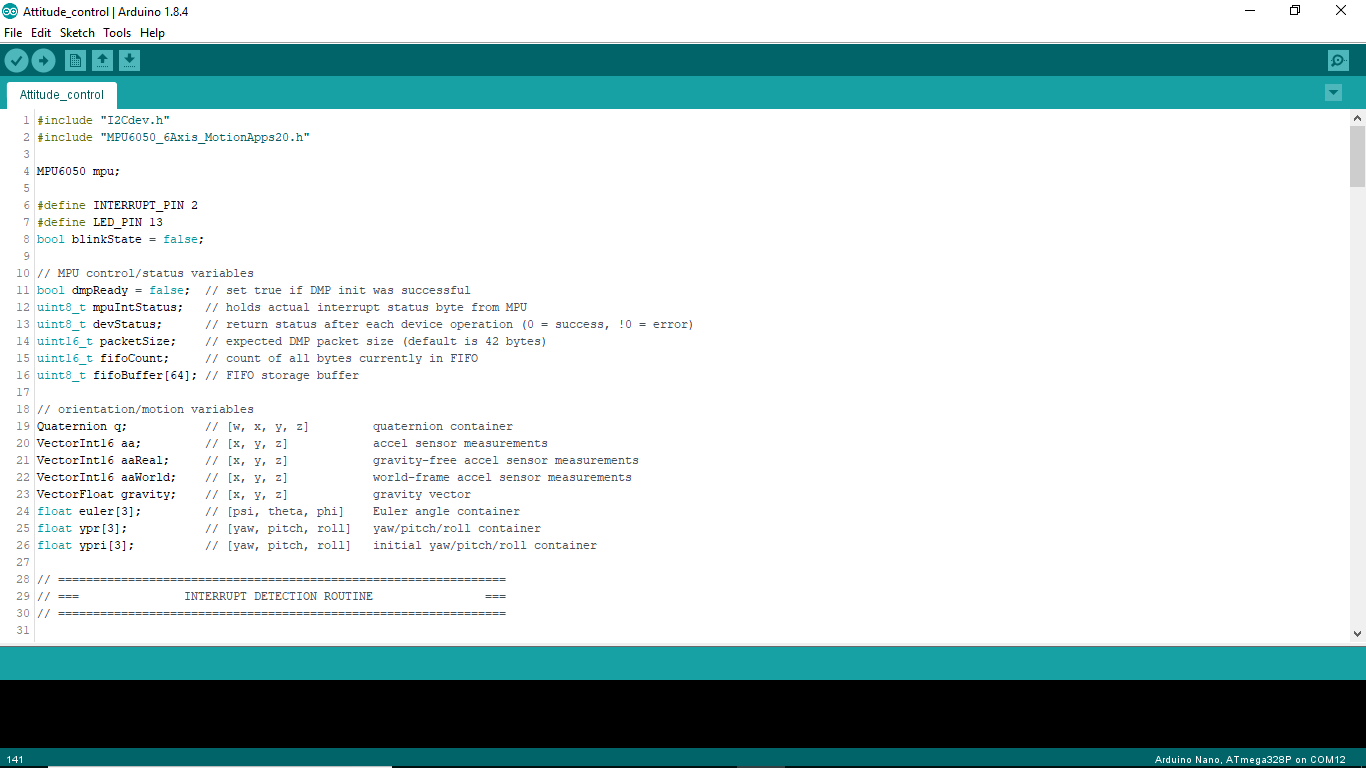
\includegraphics[width=175mm,height=135mm]{23.jpg}
\newpage
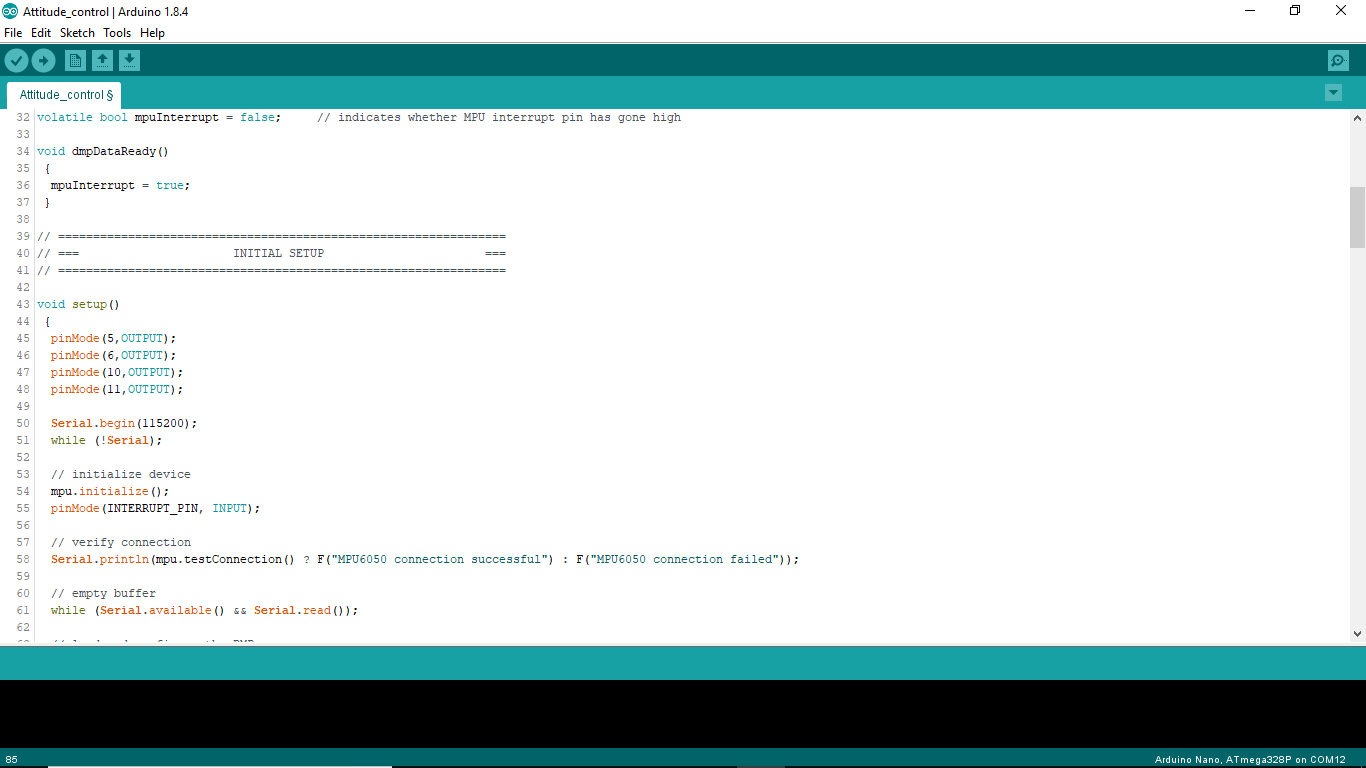
\includegraphics[width=175mm,height=165mm]{24.jpg}
\newpage
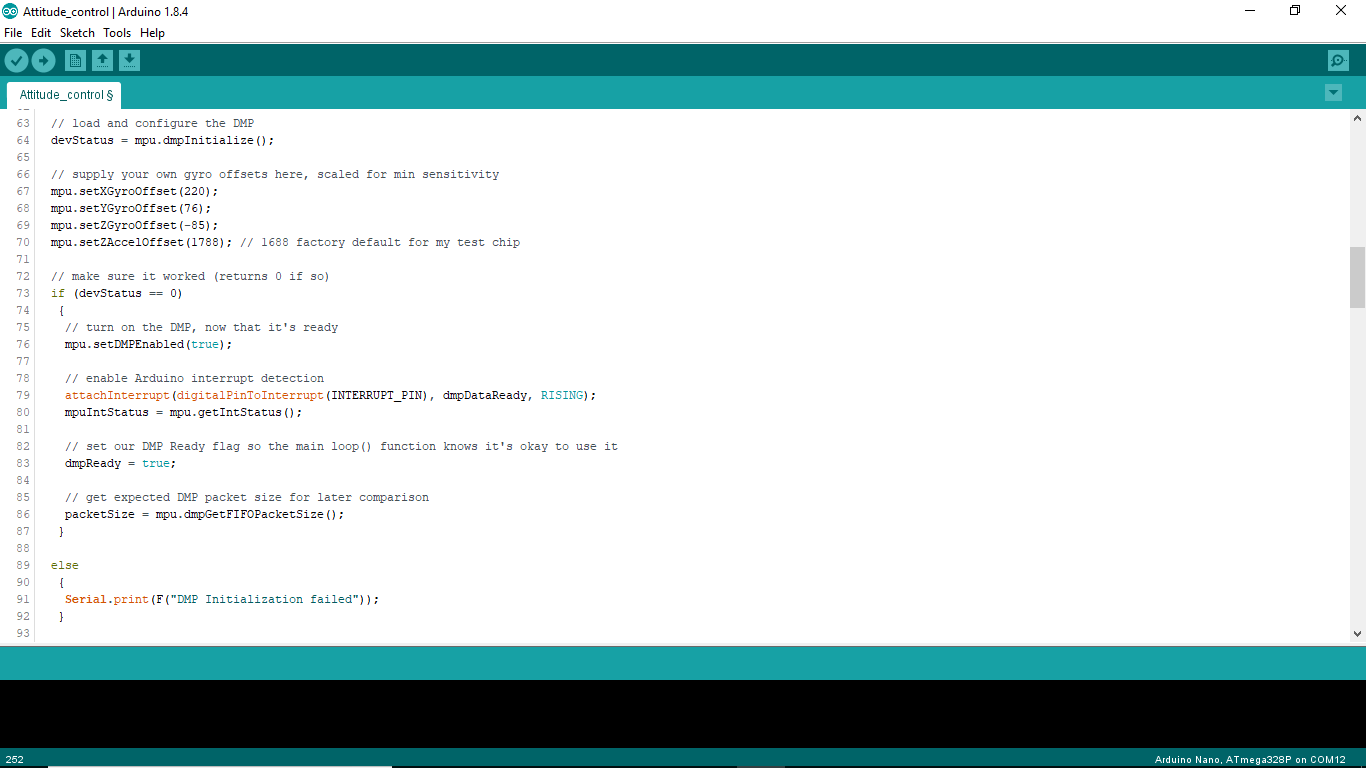
\includegraphics[width=175mm,height=165mm]{25.jpg}
\newpage
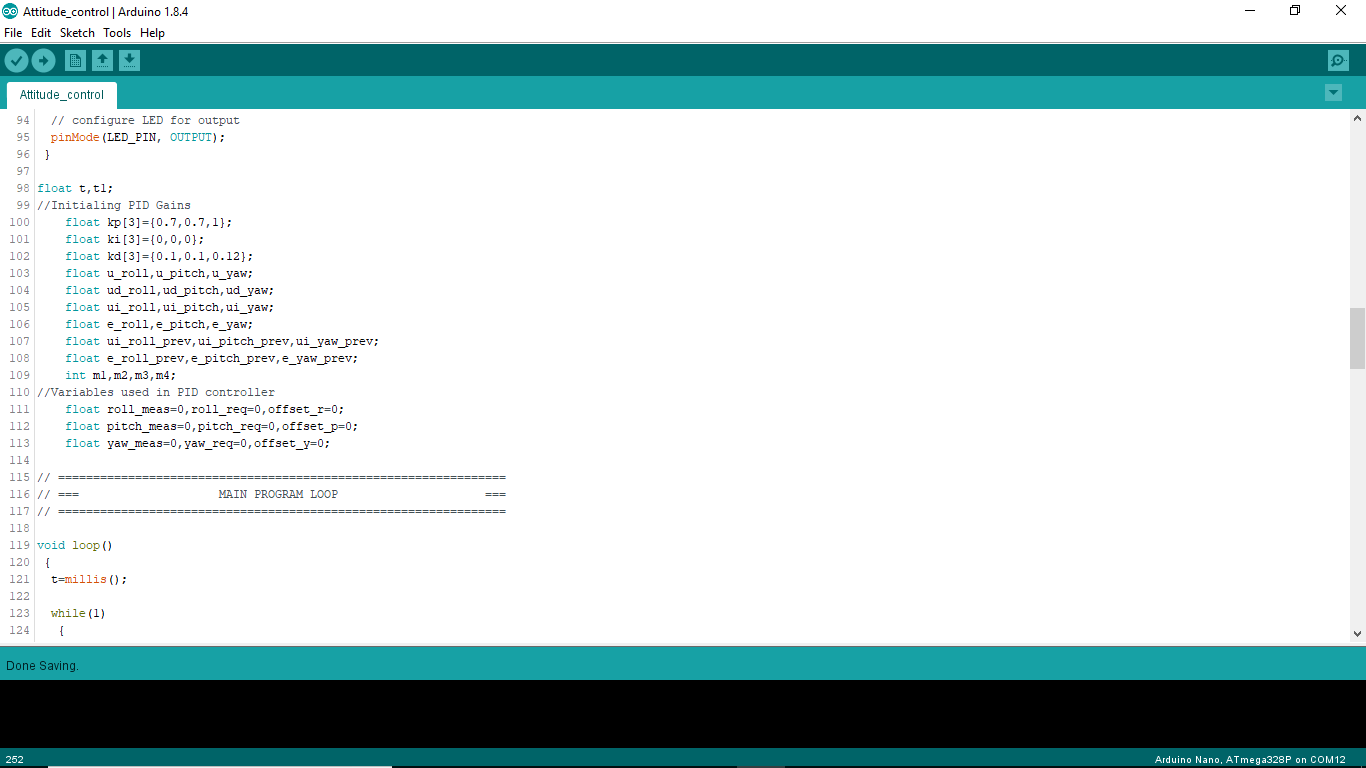
\includegraphics[width=175mm,height=165mm]{26.jpg}
\newpage
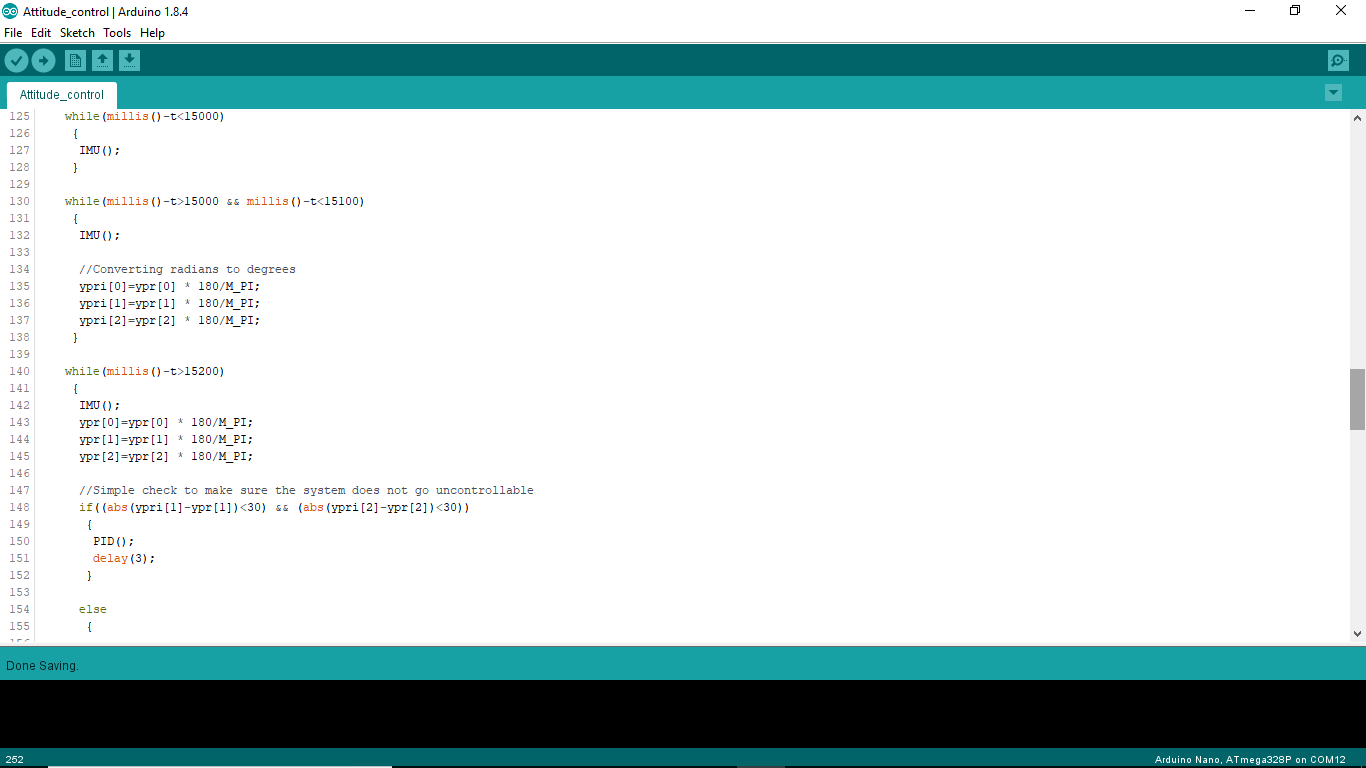
\includegraphics[width=175mm,height=165mm]{27.jpg}
\newpage
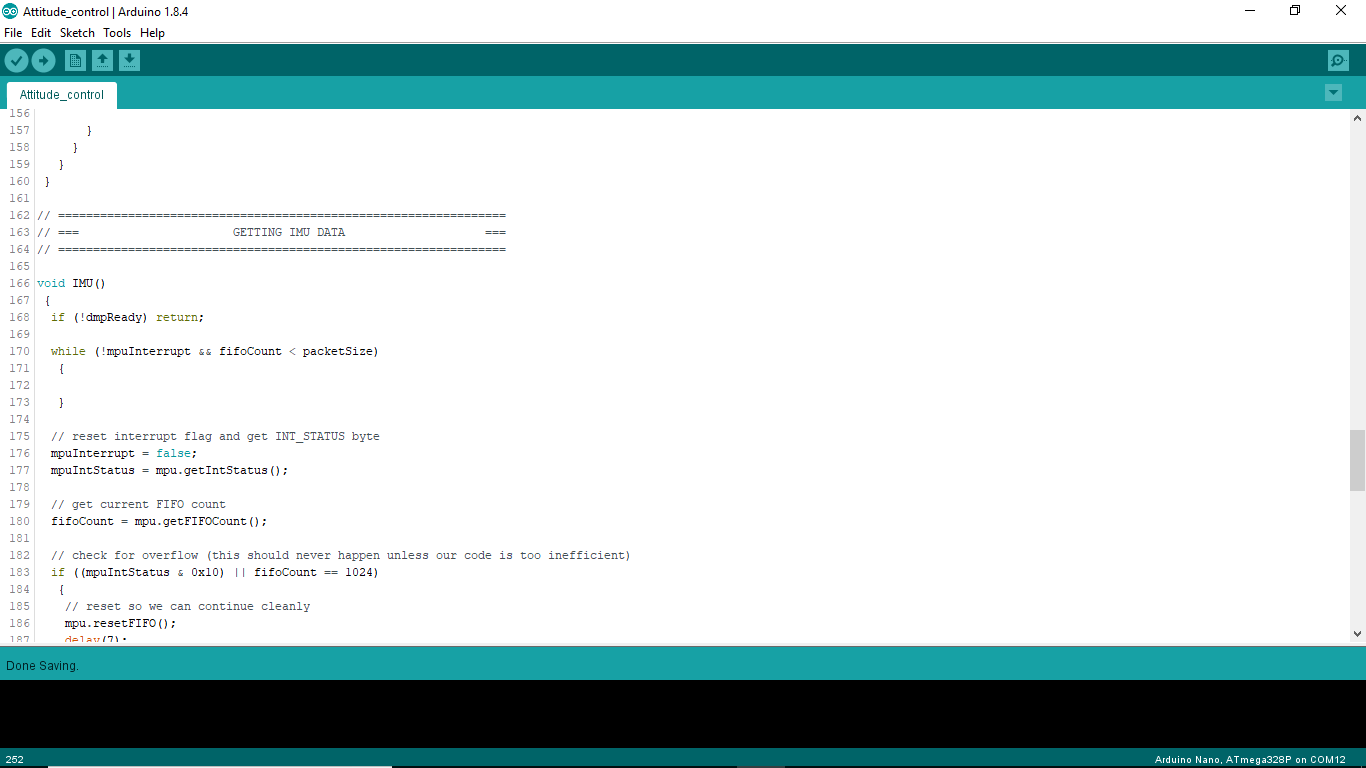
\includegraphics[width=175mm,height=165mm]{28.jpg}
\newpage
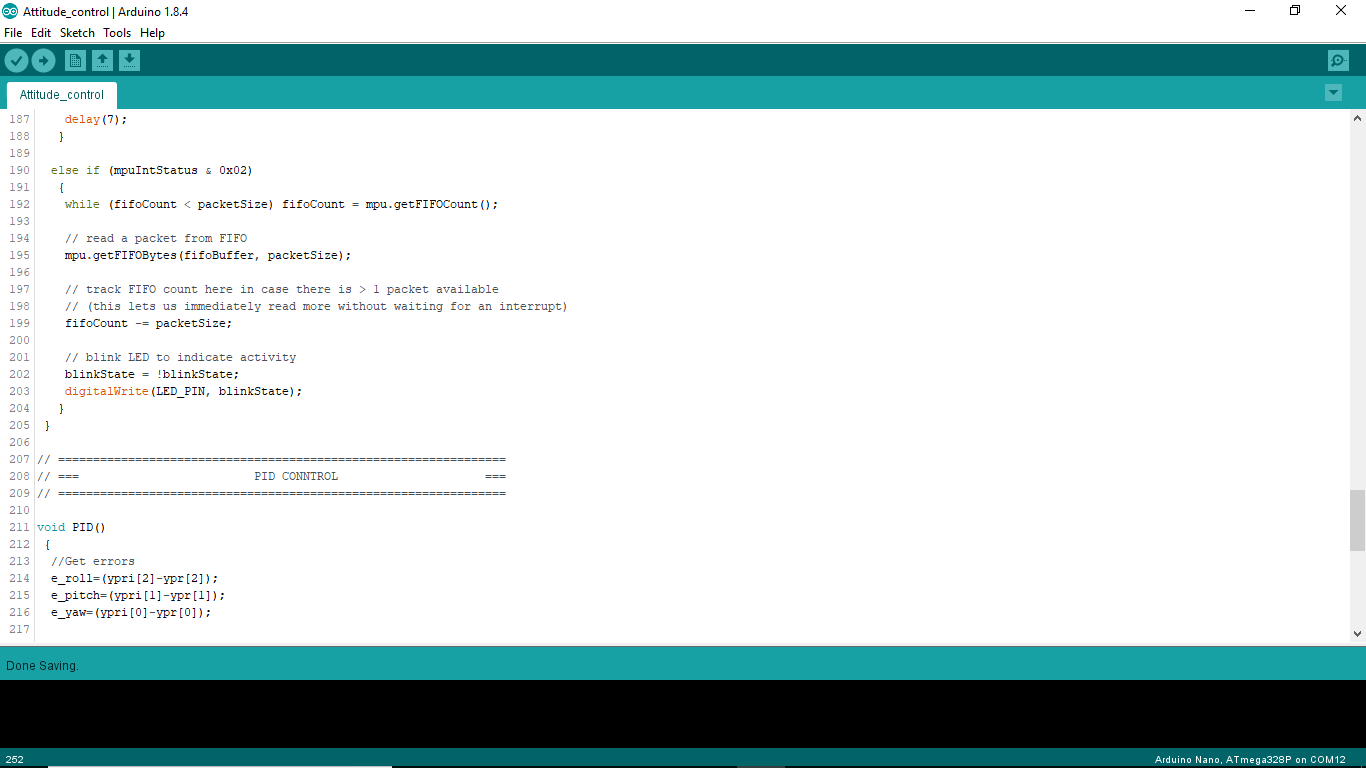
\includegraphics[width=175mm,height=165mm]{29.jpg}
\newpage
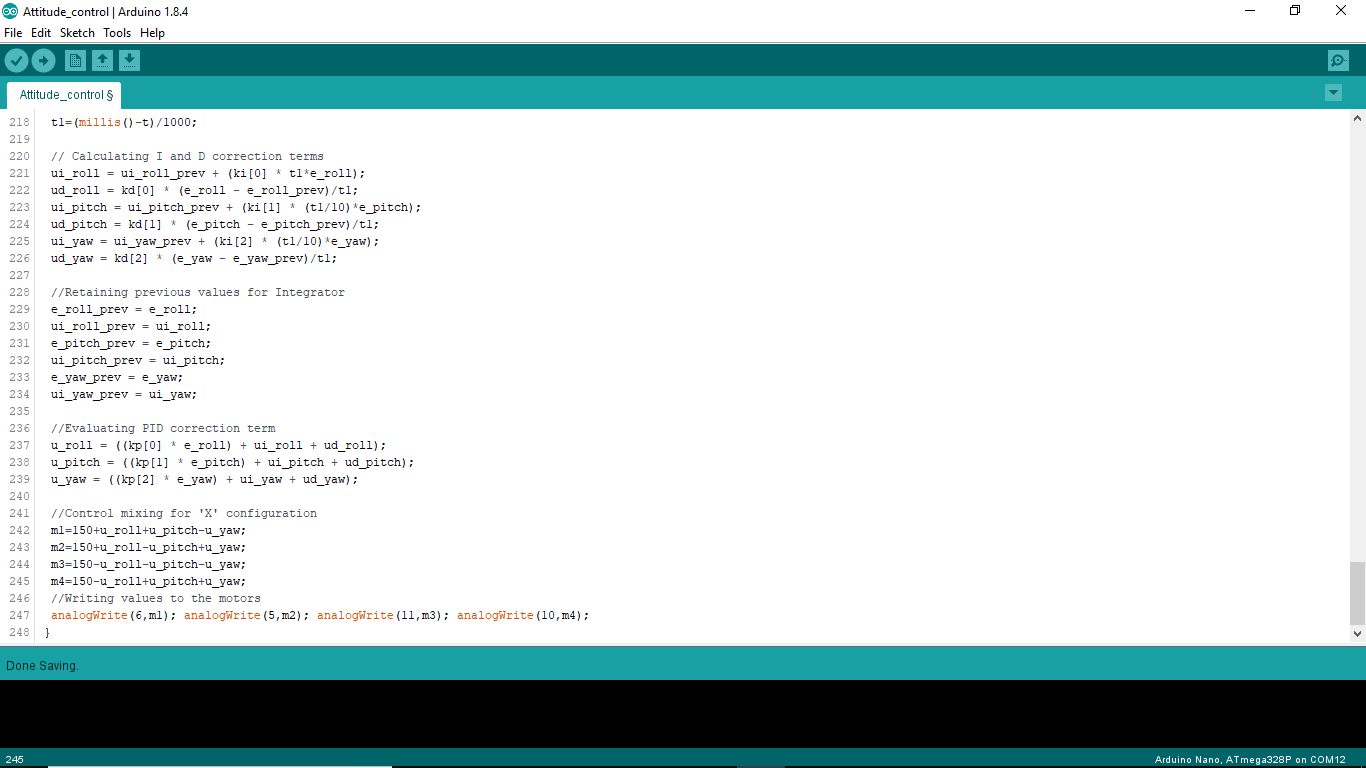
\includegraphics[width=175mm,height=165mm]{30.jpg}

\end{flushleft}

\newpage

\part{Result}

\noindent We successfully

\begin{itemize}
\item Modeled quadcopter for attitude control with graphs and animation as output.
\item Implemented parallel PID using Arduino Nano as microcontroller and MPU6050 as sensor for feedback.
\item Designed $3$ DOF test rig.
\item Verified working for yaw stabilization to counter disturbance inputs.
\end{itemize}

\noindent We failed to

\begin{itemize}
\item Verify working for roll and pitch stabilization to counter disturbance inputs.
\end{itemize}

\part{Conclusion}

\section{Learning experience}
This project helped us understand and appreciate the process of designing and implementing a controller in a practical scenario. We fully understood the working of a quadcopter which is one of the most famous applications of control theory. We got to work with features in MATLAB and Simulink that we were previously unaware of such as the S-Function Builder and the ability to represent output as an animation. Working with the MPU6050 and comparing it's performance with other IMUs taught us many new things about them. Designing the test rig for the quadcopter was an interesting experience. Designing and experimenting with different driver circuits for coreless motors was a good learning experience during which we has our first attempt at SMD level fabrication. Seeing the controller in action was also a very satisfying result.

\section{Failure log and future scope}
We have identified the main difficulty to be a disproportionate power to weight ratio. This was expected to be a challenge as designing a micro quad rotor is much harder than a regular sized one but we definitely underestimated its complexity. The hardest part was designing a driver circuit that was small, light and still capable of powering 4 motors that draw reasonably high currents and this is where we failed since we were fixated on having a driver and controller that could be mounted on a small $5x5$ cm form factor. The L293 is slightly under-powered for this application and the Si2302 despite being ideal for this use case is available only in surface mount package so testing the design before printing was impossible, but we went ahead with it anyway. The driver worked but did not perform any better than the L293. This could be due to some mistake in design or the tracks on the PCB being too thin for the high current the motors drew (despite us taking that into consideration). In conclusion, a perfect driver circuit would have lead to a perfect execution of this project and that is the primary scope for improvement. Once that is done the next step would be to replace the Arduino Nano with a NodeMCU and send commands to the drone wirelessly. Once satisfied with this, an RC application can be designed and the drone can be removed from the test rig and will be capable of flight.

\bibliographystyle{ieeetran}
\bibliography{references}

\end{document}